\chapter{भौतिकी में कृत्रिम बुद्धिमत्ता}
\label{ch:physics}

\lakshyaheading
\begin{itemize}[leftmargin=1.4em]
  \item यह समझना कि भौतिकी मूलतः एक \emph{डेटा-विज्ञान (data science)} है।
  \item मापन (measurement), त्रुटि (error) एवं data के बीच सम्बन्ध।
  \item वक्र-संयोजन (curve fitting) एवं \term{समाश्रयण}{regression} द्वारा data से
        नियम (law) खोजना - जो भौतिकी में ML का हृदय है।
  \item कण भौतिकी (particle physics) एवं खगोल विज्ञान में पैटर्न-पहचान।
  \item मोबाइल सेंसर एवं Python की सहायता से वास्तविक data पर AI का प्रयोग।
\end{itemize}

\section{भौतिकी एक डेटा-विज्ञान है}

प्रत्येक भौतिक प्रयोग में हम कोई न कोई राशि मापते हैं - समय, दूरी, ताप, वोल्टता या
बल। ये सभी मान मिलकर \eterm{data} बनाते हैं। भौतिकी का मूल कार्य इन्हीं मानों में
छिपे \eterm{pattern} खोजकर एक \term{नियम}{law} तक पहुँचना है।

उदाहरण के लिए, गैलीलियो ने झुके हुए तल (inclined plane) पर लुढ़कती गेंद के समय एवं
दूरी के अनेक मान लिए, और उनमें यह pattern पहचाना कि $s \propto t^2$। यह ठीक वही कार्य है
जो आज एक Machine Learning model करता है - \emph{data से नियम सीखना}। अंतर केवल इतना है कि
गैलीलियो ने यह स्वयं किया, जबकि अब विशाल data पर यह कार्य मशीन तेज़ी से कर देती है।

\begin{jante}
सन् 2017 में खगोलविदों ने Google की एक \emph{neural network} की सहायता से NASA की
Kepler दूरबीन के पुराने data में दो नए ग्रह (\emph{exoplanets} - Kepler-90i तथा
Kepler-80g) खोजे, जिन्हें मनुष्य पहले चूक गए थे। मशीन ने वही प्रकाश-वक्र (light curve)
देखे, पर बहुत महीन pattern पकड़ लिया।
\end{jante}

\section{मापन, त्रुटि एवं data}

कोई भी मापन पूर्णतः सटीक नहीं होता - हर माप में कुछ \term{त्रुटि}{error} रहती है।
इसीलिए भौतिकी में एक ही राशि को कई बार मापा जाता है। इन मानों का \emph{माध्य (mean)}
सत्य के निकट होता है और उनका फैलाव (spread) त्रुटि का संकेत देता है।

\begin{itemize}[leftmargin=1.4em]
  \item \term{क्रमबद्ध त्रुटि}{Systematic error} - हर बार एक ही दिशा में (जैसे ग़लत
        अंशांकित स्केल)।
  \item \term{यादृच्छिक त्रुटि}{Random error} - हर बार बदलती हुई (जैसे प्रतिक्रिया-समय)।
\end{itemize}

AI के लिए यह बहुत महत्वपूर्ण है: यदि data में बहुत अधिक यादृच्छिक त्रुटि है (अर्थात्
data ``शोरयुक्त'' / \emph{noisy} है), तो model का पूर्वानुमान भी अनिश्चित होगा। इसीलिए
कहा जाता है - \emph{``अच्छा data ही अच्छी भौतिकी एवं अच्छी AI की नींव है।''}

\begin{sochiye}
यदि आप किसी लोलक (pendulum) का दोलन-काल केवल एक बार मापें बनाम 20 दोलनों का समय
मापकर उसे 20 से भाग दें - तो किसमें त्रुटि कम होगी और क्यों? यही विचार ML में ``अधिक
data से बेहतर परिणाम'' के सिद्धांत से कैसे जुड़ता है?
\end{sochiye}

\section{data से नियम: समाश्रयण (Regression)}

मान लीजिए आपके पास किसी प्रयोग के कुछ बिंदु (data points) हैं और आप उनके बीच से
सर्वोत्तम रेखा खींचना चाहते हैं। इस रेखा को खोजने की विधि को \term{रैखिक समाश्रयण}{Linear
Regression} कहते हैं। यह Machine Learning का सबसे सरल एवं सबसे महत्वपूर्ण model है।

रेखा का समीकरण होता है:
\[
  y = m x + c
\]
जहाँ $m$ ढलान (slope) तथा $c$ अंतःखंड (intercept) है। ML का कार्य ऐसे $m$ एवं $c$
खोजना है जिससे रेखा से बिंदुओं की लम्बवत् दूरियों के वर्गों का योग (कुल त्रुटि)
न्यूनतम हो। इसी ``वर्गों के योग को न्यूनतम करने'' के विचार को \term{अल्पतम वर्ग
विधि}{Least Squares Method} कहते हैं।

\begin{table}[h]
\centering
\begin{tabular}{@{}p{5cm} p{8cm}@{}}
\toprule
\rowcolor{cvBlue}\hdc{भौतिकी का प्रयोग} & \hdc{समाश्रयण किस नियम को ``सीखता'' है} \\
\midrule
स्प्रिंग पर बल बनाम विस्तार & हुक का नियम (Hooke's law), $F = kx$ \\
ओम का परिपथ (V बनाम I)      & ओम का नियम, $V = IR$ \\
गर्म वस्तु का ताप बनाम समय  & शीतलन (cooling) की प्रवृत्ति \\
\bottomrule
\end{tabular}
\caption{रैखिक समाश्रयण से भौतिकी के नियमों की पहचान}
\end{table}

ध्यान दें - model ``नियम'' को पहले से नहीं जानता; वह केवल data देखकर सर्वोत्तम $m$ एवं
$c$ निकालता है। यही ``data से सीखना'' का सार है। चित्र~\ref{fig:regression} में बिखरे
हुए डेटा-बिंदु एवं उनसे होकर गुज़रती सर्वोत्तम रेखा दिखाई गई है।

\begin{figure}[h]
\centering
\begin{tikzpicture}
\begin{axis}[
    width=10cm, height=6.2cm,
    font=\sffamily\small,
    xlabel={विस्तार $x$ (cm)}, ylabel={बल $F$ (N)},
    xmin=0, xmax=12, ymin=0, ymax=6,
    grid=both, grid style={aigrey!20},
    axis lines=left,
    legend pos=north west, legend cell align=left,
]
% डेटा-बिंदु (scatter)
\addplot[only marks, mark=*, aiblue, mark size=2.4pt]
  coordinates {(2,1.0) (4,2.1) (6,2.9) (8,4.2) (10,5.0)};
\addlegendentry{data}
% सर्वोत्तम रेखा (best-fit), लगभग F = 0.505 x
\addplot[thick, red, domain=0:11] {0.505*x + 0.01};
\addlegendentry{सर्वोत्तम रेखा (best-fit)}
\end{axis}
\end{tikzpicture}
\caption{रैखिक समाश्रयण (linear regression): बिखरे डेटा-बिंदुओं से होकर least-squares
द्वारा खींची गई सर्वोत्तम रेखा।}
\label{fig:regression}
\end{figure}

\begin{gatividhi}[हाथ से ``regression'' - सर्वोत्तम रेखा]
\textbf{लक्ष्य:} बिना कंप्यूटर के यह अनुभव करना कि model सर्वोत्तम रेखा कैसे खोजता है।\\[4pt]
\textbf{सामग्री:} ग्राफ़ पेपर, पैमाना, पेंसिल।\\[4pt]
\textbf{चरण:}
\begin{enumerate}[leftmargin=1.6em]
  \item किसी स्प्रिंग पर अलग-अलग भार लटकाकर विस्तार (extension) मापें - कम से कम 6 मान।
  \item बल ($F$) बनाम विस्तार ($x$) के बिंदु ग्राफ़ पर अंकित करें।
  \item आँख से ऐसी सीधी रेखा खींचें जो अधिकतम बिंदुओं के निकट हो (best-fit line)।
  \item रेखा की ढलान ($m$) निकालें - यही स्प्रिंग नियतांक (spring constant) $k$ है।
\end{enumerate}
\textbf{अवलोकन:} आपने जो किया, कंप्यूटर वही ``least squares'' से अधिक सटीकता से करता है।
\end{gatividhi}

\section{भौतिकी data पर Python (एक झलक)}

ऊपर की रेखा कंप्यूटर से खींचना बहुत सरल है। नीचे \emph{Google Colab} में चलने वाला एक
छोटा सा Python कोड है जो data पर सर्वोत्तम रेखा निकाल देता है। (यहाँ इसे समझना पर्याप्त
है; चलाना अध्याय~5 में सीखेंगे।)

\begin{lstlisting}
import numpy as np

# experiment data: force F (newton) vs extension x (metre)
x = np.array([0.02, 0.04, 0.06, 0.08, 0.10])   # extension
F = np.array([1.0, 2.1, 2.9, 4.2, 5.0])        # force

# best-fit line F = m*x + c   (degree 1 = straight line)
m, c = np.polyfit(x, F, 1)
print("spring constant k =", round(m, 2), "N/m")
\end{lstlisting}
\colabnb{https://colab.research.google.com/github/kkreboot/ai-in-science-hindi/blob/main/notebooks/ch2-spring.ipynb}

\noindent यहाँ \texttt{np.polyfit} ही least-squares regression कर रहा है - मात्र एक
पंक्ति में वही कार्य जो आपने गतिविधि में हाथ से किया था।

\section{पैटर्न-पहचान: कण भौतिकी एवं खगोल}

कुछ भौतिक प्रयोगों में data इतना विशाल होता है कि मनुष्य उसे देख ही नहीं सकता।

\subsection{कण भौतिकी (Particle Physics)}
\emph{CERN} के \eterm{Large Hadron Collider (LHC)} में प्रति सेकंड
लगभग एक अरब ($\approx 1$ billion) कण-टकराव (collisions) होते हैं। इनमें से अधिकांश साधारण हैं; केवल कुछ दुर्लभ
घटनाएँ (rare events) महत्वपूर्ण होती हैं। AI इन्हें छाँटकर वैज्ञानिकों तक पहुँचाती है।
सन् 2012 में \emph{Higgs boson} की खोज में भी ऐसी ही पैटर्न-पहचान तकनीकों का योगदान था।

\subsection{गुरुत्वीय तरंगें (Gravitational Waves)}
\emph{LIGO} वेधशाला अत्यंत क्षीण संकेतों को मापती है। दो ब्लैक होल के टकराने से उठी
तरंग का संकेत इतना कमज़ोर होता है कि वह ``शोर'' (noise) में दब जाता है। AI एवं
पैटर्न-मिलान (pattern matching) इन तरंगों को शोर से अलग पहचानने में सहायता करते हैं।

\subsection{खगोल विज्ञान (Astronomy)}
दूरबीनें (telescopes) प्रतिदिन लाखों आकाशीय पिंडों के चित्र भेजती हैं। AI इन विशाल
छवियों में आकाशगंगाओं (galaxies), तारों एवं दुर्लभ खगोलीय घटनाओं को स्वतः पहचान एवं
वर्गीकृत कर लेती है -- जिसे हाथ से करना असंभव होता। चित्र~\ref{fig:hubble} में हबल
दूरबीन द्वारा ली गई असंख्य दूरस्थ आकाशगंगाओं की एक झलक है।

\begin{figure}[h]
\centering
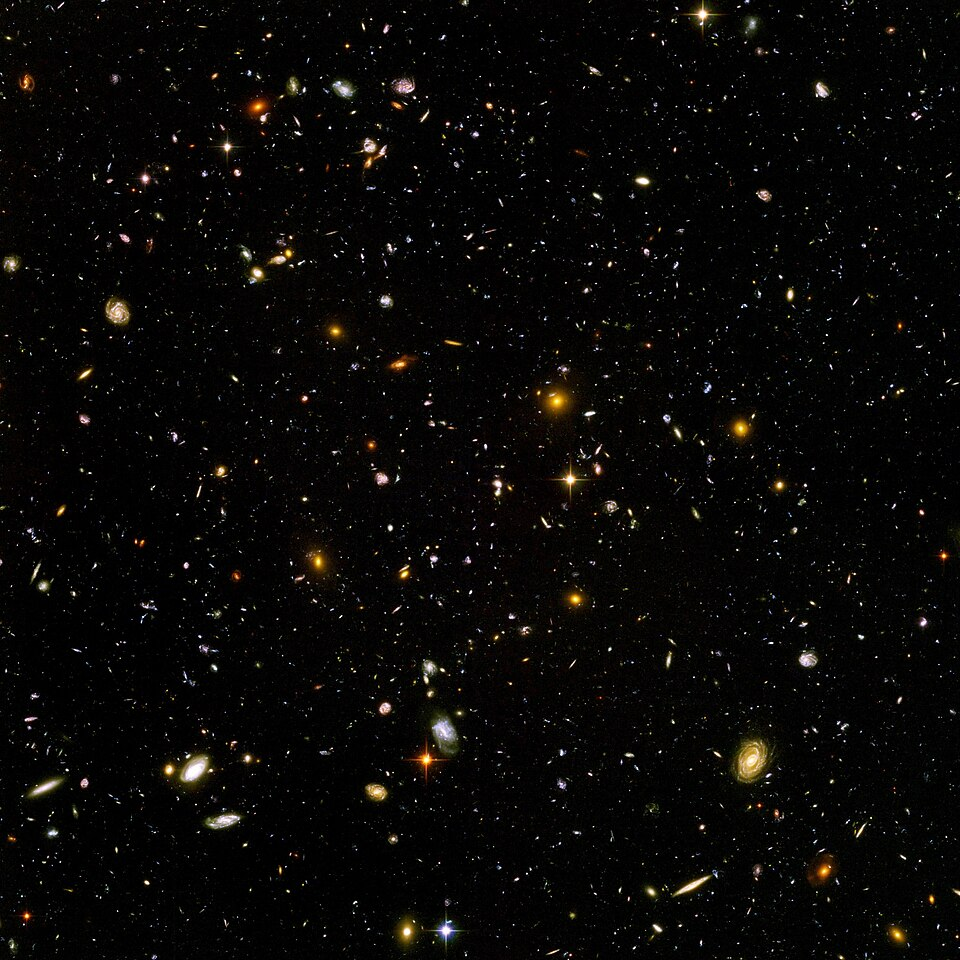
\includegraphics[width=0.62\linewidth]{images/hubble-udf.jpg}
\caption[हबल अल्ट्रा डीप फ़ील्ड -- हज़ारों आकाशगंगाएँ]{हबल अल्ट्रा डीप फ़ील्ड -- एक छोटे
से आकाश-क्षेत्र में हज़ारों आकाशगंगाएँ; AI ऐसी छवियों के विश्लेषण में सहायक
है।\imgsrc{NASA \& ESA, Wikimedia Commons (Public Domain)}}
\label{fig:hubble}
\end{figure}

\begin{jante}
\textbf{भारतीय योगदान: चंद्रयान-3 एवं ISRO (ISRO's Chandrayaan-3):}
भारतीय अंतरिक्ष अनुसंधान संगठन (ISRO) ने चंद्रयान-3 के 'प्रज्ञान रोवर' (Pragyan Rover) द्वारा भेजे गए चंद्र-सतह के चित्रों के विश्लेषण के लिए AI और कंप्यूटर विज़न (Computer Vision) का उपयोग किया। AI एल्गोरिदम रोवर के पथ में आने वाले गड्ढों (craters) और पत्थरों को स्वतः पहचानकर उसे सुरक्षित मार्ग पर बढ़ने में सहायता करते हैं। इसके अतिरिक्त, चंद्र-सतह के डिजिटल एलिवेशन model (Digital Elevation Models, DEM) बनाने में भी AI का महत्वपूर्ण योगदान रहा है।
\end{jante}

\begin{jante}
LHC प्रति सेकंड लगभग 1 \emph{petabyte} (दस लाख गीगाबाइट) data बनाता है - इसे संभालना
केवल AI एवं स्वचालित (automated) फ़िल्टर से ही सम्भव है।
\end{jante}

\section{पूर्वानुमान: गति एवं मौसम}

जब हम कुछ मापे गए मानों से अगली स्थिति का अनुमान लगाते हैं, उसे \term{पूर्वानुमान}{prediction}
कहते हैं।

\begin{itemize}[leftmargin=1.4em]
  \item \textbf{गति:} किसी प्रक्षेप्य (projectile) के कुछ बिंदु देकर उसका अगला पथ
        बताया जा सकता है - जैसे क्रिकेट में DRS की ``ball-tracking'' तकनीक।
  \item \textbf{मौसम:} तापमान, दाब एवं आर्द्रता के विशाल data से AI मौसम का
        पूर्वानुमान (weather forecasting) करती है। आधुनिक model अब पारंपरिक भौतिक
        समीकरणों के साथ-साथ ML का भी उपयोग करते हैं।
\end{itemize}

\begin{jante}
\textbf{भारतीय योगदान: मानसून का सटीक पूर्वानुमान (Monsoon Prediction by IISc):}
भारतीय विज्ञान संस्थान (IISc), बेंगलुरु और भारतीय मौसम विज्ञान विभाग (IMD) के शोधकर्ता भारत में मानसून की वर्षा के अधिक सटीक पूर्वानुमान के लिए कृत्रिम बुद्धिमत्ता (AI) और मशीन लर्निंग (ML) model का उपयोग कर रहे हैं। मानसून एक अत्यंत जटिल प्रणाली है जिसमें समुद्र के तापमान, हवा की दिशा और वायुमंडलीय दाब के बीच जटिल संबंध होते हैं। पारंपरिक सुपरकंप्यूटर भौतिक मॉडलों में जब Deep Learning को मिलाया जाता है, तो भारी वर्षा और अचानक आने वाली बाढ़ (flash floods) के पूर्वानुमान की सटीकता बहुत बढ़ जाती है।
\end{jante}

\begin{gatividhi}[मोबाइल सेंसर से वास्तविक भौतिक data]
\textbf{लक्ष्य:} वास्तविक भौतिक data एकत्र कर उसमें pattern देखना।\\[4pt]
\textbf{सामग्री:} स्मार्टफ़ोन, मुफ़्त ``Phyphox'' ऐप।\\[4pt]
\textbf{चरण:}
\begin{enumerate}[leftmargin=1.6em]
  \item ``Phyphox'' इंस्टॉल करें और ``Acceleration (without g)'' प्रयोग चुनें।
  \item फ़ोन को हाथ में लेकर धीरे ऊपर-नीचे घुमाएँ; data रिकॉर्ड करें।
  \item data को CSV रूप में निर्यात (export) करें और ग्राफ़ देखें।
  \item बताएँ - किस क्षण त्वरण (acceleration) अधिकतम था? ग्राफ़ का आकार आवर्ती
        (periodic) है या नहीं?
\end{enumerate}
\textbf{विस्तार:} यही CSV data Colab में खोलकर उस पर regression आज़माया जा सकता है।
\end{gatividhi}

\begin{figure}[h]
\centering
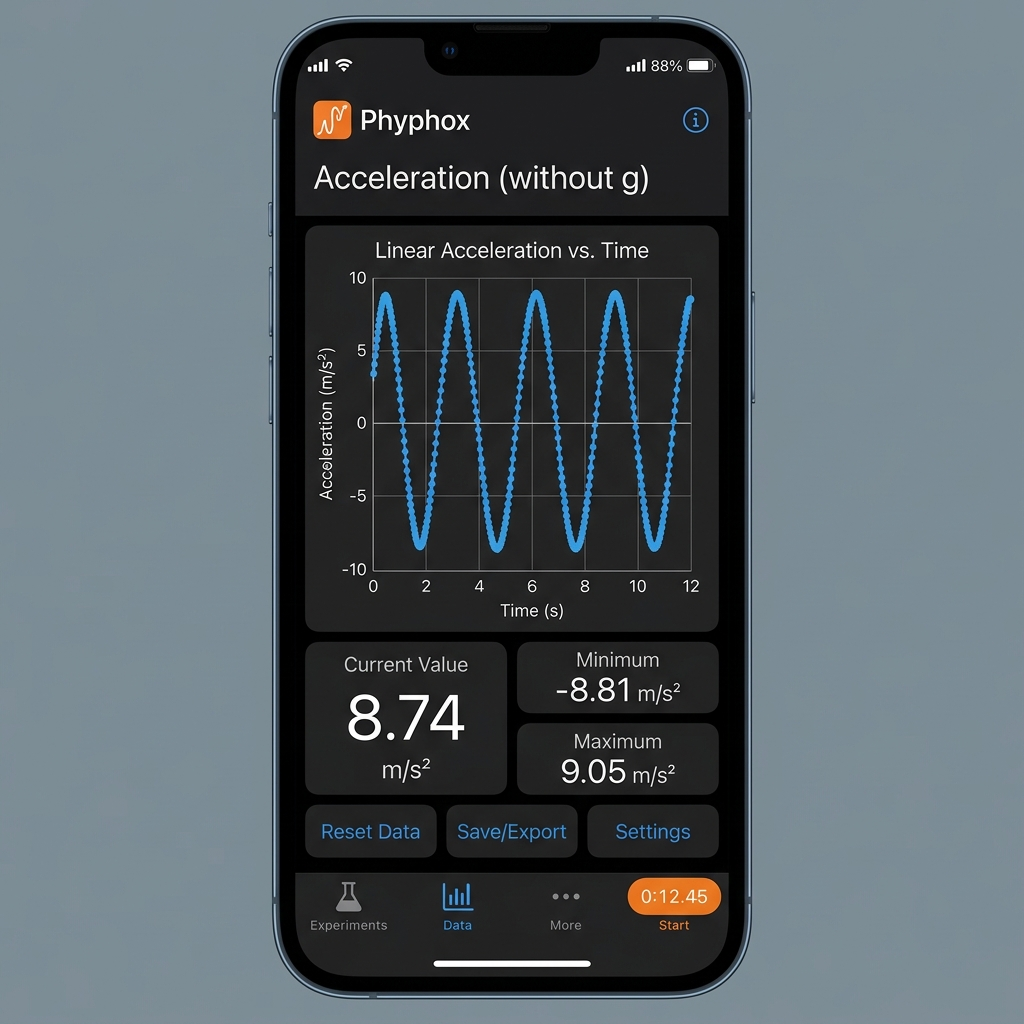
\includegraphics[width=0.48\linewidth]{images/phyphox_ui.jpg}
\caption[फिफॉक्स मोबाइल सेंसर इंटरफ़ेस]{स्मार्टफ़ोन में फिफॉक्स (Phyphox) ऐप का इंटरफ़ेस -- जहाँ त्वरण (acceleration) data को मापा और ग्राफ़ के रूप में देखा जा सकता है।}
\label{fig:phyphox-ui}
\end{figure}

% ---------------- परियोजना ----------------
\begin{pariyojana}[लोलक का दोलन-काल - मापन से पूर्वानुमान]
\textbf{उद्देश्य:} data से नियम सीखकर पूर्वानुमान करना, और उसे भौतिक सूत्र से जाँचना।\\[4pt]
\textbf{सामग्री:} धागा, छोटा भार (bob), पैमाना, स्टॉपवॉच (मोबाइल)।\\[4pt]
\textbf{कार्य (समूह में, 3–4 विद्यार्थी):}
\begin{enumerate}[leftmargin=1.6em]
  \item लोलक की लम्बाई $L$ को 6–7 भिन्न मानों पर लें (जैसे 20, 30, 40 \dots cm)।
  \item प्रत्येक लम्बाई पर 20 दोलनों का समय मापकर दोलन-काल $T$ निकालें।
  \item $T^2$ बनाम $L$ का ग्राफ़ बनाएँ - यह एक सीधी रेखा आनी चाहिए।
  \item रेखा से किसी \emph{नई} लम्बाई (जो आपने मापी नहीं) के लिए $T$ का पूर्वानुमान करें।
  \item अब वास्तव में उस लम्बाई पर मापकर देखें - पूर्वानुमान कितना सही था?
  \item परिणाम की तुलना सूत्र $T = 2\pi\sqrt{L/g}$ से करें तथा ग्राफ़ की ढलान से
        $g$ का मान निकालें।
\end{enumerate}
\textbf{मूल्यांकन:} data की शुद्धता, ग्राफ़, पूर्वानुमान की त्रुटि एवं $g$ के मान की
यथार्थता (accuracy) के आधार पर।
\end{pariyojana}

% ---------------- सारांश ----------------
\begin{bharatai}
पुणे का \textbf{GMRT} (विशाल रेडियो दूरबीन) एवं \textbf{AstroSat} जैसी भारतीय वेधशालाओं
से मिलने वाले विशाल खगोलीय data के विश्लेषण एवं पैटर्न-पहचान में AI का उपयोग बढ़ रहा है।
\end{bharatai}

\section*{सारांश (Summary)}
\addcontentsline{toc}{section}{सारांश}
\begin{itemize}[leftmargin=1.4em]
  \item भौतिकी मूलतः मापन एवं data पर आधारित विज्ञान है; नियम खोजना data में pattern
        खोजना ही है।
  \item हर मापन में त्रुटि रहती है; अधिक एवं स्वच्छ data बेहतर परिणाम देता है।
  \item रैखिक समाश्रयण (linear regression) data से नियम ``सीखने'' का सरलतम ML model है,
        जो least-squares द्वारा सर्वोत्तम रेखा खोजता है।
  \item कण भौतिकी, गुरुत्वीय तरंगों एवं खगोल में AI विशाल data से दुर्लभ pattern पहचानती है।
  \item मोबाइल सेंसर एवं Python जैसे मुफ़्त उपकरणों से विद्यार्थी स्वयं यह अनुभव कर सकते हैं।
\end{itemize}

% ---------------- अभ्यास ----------------
\section*{अभ्यास (Exercises)}
\addcontentsline{toc}{section}{अभ्यास}
\textbf{अ. रिक्त स्थान भरिए:}
\begin{enumerate}[leftmargin=1.6em]
  \item data में से सर्वोत्तम रेखा खोजने की ML विधि को \rule{2.8cm}{0.4pt} कहते हैं।
  \item सर्वोत्तम रेखा वह है जिससे बिंदुओं की कुल \rule{2.8cm}{0.4pt} न्यूनतम हो।
  \item हर बार एक ही दिशा में होने वाली त्रुटि \rule{2.8cm}{0.4pt} त्रुटि कहलाती है।
\end{enumerate}

\textbf{ब. लघु उत्तरीय:}
\begin{enumerate}[leftmargin=1.6em]
  \item ``भौतिकी एक डेटा-विज्ञान है'' - इस कथन को गैलीलियो के उदाहरण से समझाइए।
  \item रैखिक समाश्रयण किसी भौतिक नियम को कैसे ``सीखता'' है? एक उदाहरण दीजिए।
  \item कण भौतिकी (LHC) में AI क्यों आवश्यक है? संक्षेप में लिखिए।
\end{enumerate}

\textbf{स. क्रियात्मक / दीर्घ उत्तरीय:}
\begin{enumerate}[leftmargin=1.6em]
  \item स्प्रिंग वाली गतिविधि कीजिए और बताइए कि ढलान से स्प्रिंग नियतांक $k$ कैसे
        प्राप्त होता है।
  \item दिए गए data - $x:(1,2,3,4)$ तथा $y:(2,4,6,8)$ - के लिए हाथ से $m$ एवं $c$
        ज्ञात कीजिए। यह कौन-सा भौतिक सम्बन्ध दर्शाता है?
  \item Phyphox से एकत्र अपने त्वरण-data का ग्राफ़ बनाकर उसमें दिखने वाले pattern का
        वर्णन कीजिए।
\end{enumerate}

\begin{mcq}
  \item सरल रेखा $y=mx+c$ में $m$ क्या दर्शाता है?
    \begin{choices}\item अंतःखंड \item ढलान \item त्रुटि \item औसत\end{choices}
  \item data से सर्वोत्तम रेखा निकालने की विधि कहलाती है:
    \begin{choices}\item वर्गीकरण \item समाश्रयण (regression)
      \item क्रमबद्धन \item एन्क्रिप्शन\end{choices}
  \item गुरुत्वीय तरंगों को मापने वाली वेधशाला है:
    \begin{choices}\item LIGO \item LHC \item NASA \item ISRO\end{choices}
  \item Higgs boson की खोज किस संस्था के प्रयोग से जुड़ी है?
    \begin{choices}\item CERN \item NCBI \item PubChem \item WHO\end{choices}
\end{mcq}

\begin{mukhyashabd}
\textbf{data}, \textbf{pattern}, \textbf{नियम (law)}, \textbf{त्रुटि (error)} --
क्रमबद्ध एवं यादृच्छिक, \textbf{रैखिक समाश्रयण (Linear Regression)},
\textbf{अल्पतम वर्ग विधि (Least Squares)}, \textbf{पूर्वानुमान (prediction)},
\textbf{LHC}, \textbf{LIGO}।
\end{mukhyashabd}
\selfcheckqr{https://kkreboot.github.io/ai-in-science-hindi/quiz/ch2.html}
